\documentclass[tikz,border=5pt]{standalone}
\usepackage{amsmath}
\begin{document}

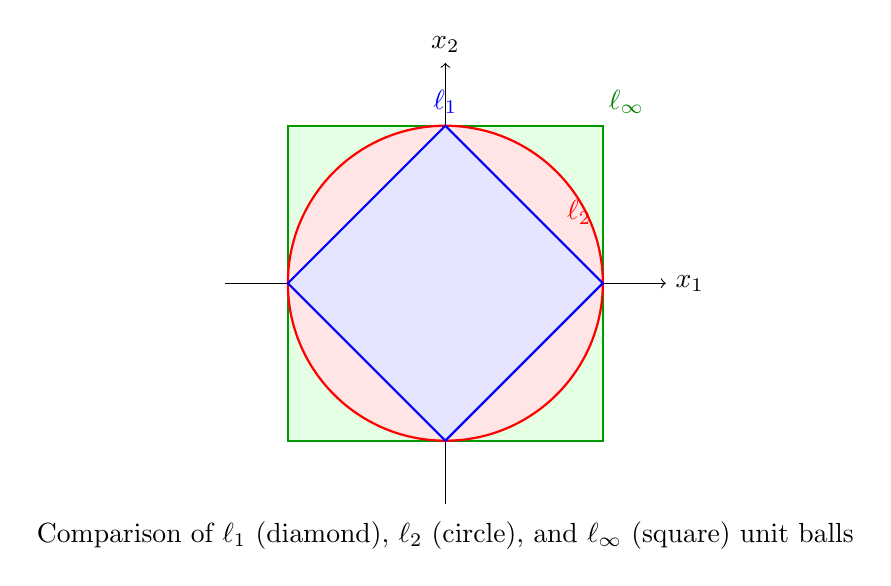
\begin{tikzpicture}[scale=2]
  % Axes
  \draw[->] (-1.4,0) -- (1.4,0) node[right] {$x_1$};
  \draw[->] (0,-1.4) -- (0,1.4) node[above] {$x_2$};

  % ℓ∞ unit ball (square)
  \draw[thick,green!60!black,fill=green!10]
    (-1,-1) rectangle (1,1);
  \node[green!50!black] at (1.15,1.15) {$\ell_\infty$};

  % ℓ₂ unit ball (circle)
  \draw[thick,red,fill=red!10] (0,0) circle (1);
  \node[red] at (0.85,0.45) {$\ell_2$};

  % ℓ₁ unit ball (diamond)
  \draw[thick,blue,fill=blue!10]
    (1,0) -- (0,1) -- (-1,0) -- (0,-1) -- cycle;
  \node[blue] at (0.0,1.15) {$\ell_1$};

  % Title / caption
  \node[below] at (0,-1.45)
    {Comparison of $\ell_1$ (diamond), $\ell_2$ (circle), and $\ell_\infty$ (square) unit balls};
\end{tikzpicture}

\end{document}
